% app0.tex (silly little file to separate chapters from appendices)
\appendix
\titleformat{\chapter}[display]   
{\normalfont\large\bfseries\centering}{\chaptertitlename\ \thechapter}{10pt}{\large}   
\titlespacing*{\chapter}{0pt}{-20pt}{25pt}
%\setcounter{secnumdepth}{1}
%\setcounter{section}{0}

\chapter{Hydrodynamics of Homogeneous Liquids}
\section{Energy Conservation Equation for the Isentropic Flow in the Potential Field}%MK, Eq.~\eqref{s_cons}.}
\label{app:s_cons}
\setcounter{equation}{0}

It is often useful to express the entropy conservation condition, \eqref{s_cons} in a form of equations satisfied by the energy per unit mass, $\epsilon$.
Note that in the presence of the external potential, $U$, the energy  $\epsilon$ includes neither the kinetic energy of the macroscopic energy of the flow nor  the potential energy in the external field.
The latter, therefore has to be included in the energy conservation equation explicitly.
Consider the element of a fluid containing the fixed amount of particles, $N$ of mass $m$ at times $t$ and $t + d t$.
Let the energy, entropy and volume change during the  considered time interval be denoted as $dE$, $dS$ and $dV$.
Then the general thermodynamic formula
\be\label{dE}
d E = T d S - p d V + \mu d N
\ee
gives for the change in the course of the isentropic  flow of a fixed mass of a fluid,
\be
D \epsilon = - p \frac{d V}{ N m}  = - \frac{ p}{\rho} \frac{ d V }{ V} 
\ee
which expresses the change in the energy per unit mass in terms of the fractional volume increment, $d V / V$.
The fractional volume increment is due to the finite divergence of the flow velocity,
\be
\frac{ d V }{d t V} = \bm{\nabla} \cdot \bm{v} \, .
\ee
And we finally obtain Eq.~\eqref{alt_s_cons1}, which thanks to
%As a result thanks to 
the continuity Eq.~\eqref{cont} under the conditions of the isentropic flow, \eqref{s_cons}, the energy density per unit mass,  satisfies the following equation,  
\be\label{alt_s_cons2}
 \frac{\partial \rho \epsilon}{\partial t } + \bm{\nabla} (\bm{v} \rho \epsilon)= -  p \bm{\nabla} \cdot \bm{v} \, ,
\ee
where $\rho \epsilon$ is the energy per unit volume.

We now demonstrate that Eq.~\eqref{alt_s_cons1} is equivalent to the energy conservation expressed in the form, Eq.~\eqref{e_cons}.
First we write it as
\be\label{alt_s_cons3}
 \frac{\partial \rho (\epsilon + v^2/2 +U/m)}{\partial t } 
 -\frac{\partial \rho (v^2/2)}{\partial t } 
 -(U/m)\frac{\partial \rho }{\partial t }
  + \bm{\nabla} [\bm{v} (\rho \epsilon + p)] - \bm{\nabla} p \cdot  \bm{v} =0 \, ,
\ee
where we have used the fact that the potential energy $U(\bm{r})$ is time independent.
The condition that is required for the energy conservation to hold. 
Now write, using the continuity equation, \eqref{cont} 
\be\label{alt_s_cons4}
\frac{\partial \rho (v^2/2)}{\partial t } =
- \bm{\nabla}\cdot ( \rho \bm{v} ) v^2/2 + \rho \partial_t v^2/2
\ee
We further have,
\be\label{alt_s_cons5}
\frac{\partial \rho (v^2/2)}{\partial t } =
- \bm{\nabla}\cdot ( \rho \bm{v}  v^2/2 ) +    \rho \bm{v} \cdot \bm{\nabla}(v^2/2 )+ \rho \bm{v} \cdot \partial_t \bm{v}
\ee
In addition we write using the continuity equation, \eqref{cont} again,
\be\label{alt_s_cons5a}
(U/m)\frac{\partial \rho }{\partial t } =- (U/m) \bm{\nabla} \cdot (\rho \bm{v} ) = -\bm{\nabla} \cdot [ (U/m) \rho \bm{v} ] + \rho \bm{v} \cdot \bm{\nabla}  ( U/m).
\ee
Substitution of Eqs.~\eqref{alt_s_cons5} and \eqref{alt_s_cons5a} to Eq.~\eqref{alt_s_cons3} gives
\begin{align}\label{alt_s_cons6}
 \frac{\partial \rho (\epsilon + U/m + v^2/2)}{\partial t } &
 + \bm{\nabla}\cdot [ \rho \bm{v} (\epsilon + U/m+ p/\rho + v^2/2 ) ] 
 \notag \\
& -   \rho \bm{v} \cdot 
 [ 
 \bm{\nabla} \cdot v^2/2 + \partial_t \bm{v}
+ (\bm{\nabla} p)/\rho + \bm{\nabla} U/m] =0 \, .
\end{align}
Since 
\be\label{vi}
 \bm{\nabla} \cdot v^2/2 = \bm{v} \times [\bm{\nabla} \times \bm{v}] + (\bm{v} \cdot \bm{\nabla }) \bm{v}
\ee
we have according to the Euler equation, \eqref{Euler1}
\begin{align}\label{alt_s_cons7}
& \bm{v} \cdot 
 [ 
 \bm{\nabla} \cdot v^2/2 + \partial_t \bm{v}
+ \bm{\nabla} p/\rho+ \bm{\nabla} U/m] 
\notag \\
& =
\bm{v} \cdot 
 [ 
 (\bm{v} \cdot \bm{\nabla }) \bm{v} + \partial_t \bm{v}
+ \bm{\nabla} p/\rho + \bm{\nabla} U/m] = 0
\end{align}
Finally, substitution of Eq.~\eqref{alt_s_cons7} in Eq.~\eqref{alt_s_cons6} yields energy conservation Eq.~\eqref{e_cons}.

\section{Thermodynamic Identities}
\label{app:FL_s}



The identity, 
\begin{align}\label{sound13}
\left(\frac{\partial P}{\partial \rho} \right)_{s} =\frac{n}{m} \left(\frac{\partial \mu}{\partial n} \right)_{s}
\end{align}

\noindent
{\it Proof:}
%Here we demonstrate the equivalence of \eqref{FL19} and the relation \eqref{s_13}.
From the thermodynamic relation \eqref{dE} we have the Maxwell relation 
\be\label{MR1}
- \left(\frac{\partial P}{\partial N} \right)_{S,V} = \left(\frac{\partial \mu}{\partial V} \right)_{S,N}\, .
\ee
As a result,
 \be\label{MR2}
\frac{V}{m} \left(\frac{\partial P}{\partial N} \right)_{S,V} = \left(\frac{\partial P}{\partial \rho} \right)_{s}\, ,\quad
\frac{V}{m} \left(\frac{\partial \mu}{\partial V} \right)_{S,N} = -\frac{N}{m} \left(\frac{\partial \mu}{\partial N} \right)_{S,V}=
 -\frac{n}{m} \left(\frac{\partial \mu}{\partial n} \right)_{s}
\ee
Equations \eqref{MR1} and \eqref{MR2} yield Eq.~\eqref{sound13}.
%MK NEW SECTION


%\section{Relation Between the Adiabatic and Isothermal Susceptibilities}
%\label{app:ratio}

Identity, Eq.~\eqref{rat},
\begin{align*}
\frac{(\partial p / \partial \rho)_s }{(\partial p / \partial \rho)_T } = \frac{c_p}{c_V}\, .
\end{align*}

%In this appendix we prove the relation \eqref{rat}.

\noindent{\it Proof:}
Let us denote the Jacobian, $J$ of transformation from the variables $(x,y)$ to the variables $(u,v)$ by 
\be
J = \frac{\partial(u,v)}{\partial(x,y)}.
\ee
Then,
\be
\frac{ \partial (p, s) }{ \partial (\rho, s)} = \frac{ \partial (p, s) }{ \partial (p, T)}  \frac{ \partial (p, T) }{ \partial (\rho, T)}  \frac{ \partial (p, T) }{ \partial (\rho, s)}.
\ee
And since
\be
\frac{ \partial (p, s) }{ \partial (\rho, s)} = \left(\frac{ \partial p}{\partial \rho}\right)_s\, , \quad \frac{ \partial (p, T) }{ \partial (\rho, T)} = \left(\frac{ \partial p}{\partial \rho}\right)_T
\ee
\be
T \frac{ \partial (p, s) }{ \partial (p, T)} = c_p\, , \quad T \frac{ \partial (\rho, s) }{ \partial (\rho, T)} = c_V
\ee
we recover Eq.~\eqref{rat}.



The identity,
\be\label{id43}
\left(\frac{ \partial p }{ \partial n} \right)_{\varepsilon} = \left(\frac{ \partial p }{ \partial n} \right)_{S} - \frac{ V}{T} \left(\frac{ \partial p }{ \partial S }\right)_{n} \frac{\varepsilon + p}{n},
\ee 
where $S$ is the entropy of the volume $V$ with $N$ particles.

\noindent {\it Proof:}
We choose to associate the change of the density $n$ with the change in the volume $V$ while keeping the number of particles, $N$ fixed.
\begin{align}\label{id44}
\left(\frac{\partial p}{\partial n}\right)_{\varepsilon} & = \frac{ \partial ( p, \varepsilon )}{\partial (n , S) }\frac{ \partial ( n, S )}{\partial (n , \varepsilon) }=
\left[
\left(\frac{\partial p}{\partial n}\right)_{S} \left(\frac{\partial \varepsilon}{\partial S}\right)_{n} 
-
\left(\frac{\partial p}{\partial S}\right)_{n} \left(\frac{\partial \varepsilon}{\partial  n}\right)_{p}
\right] 
\left( \frac{\partial S}{\partial \varepsilon}\right)_{n}
\notag \\
& 
=
\left(\frac{\partial p}{\partial n}\right)_{S} 
-
\left(\frac{\partial p}{\partial S}\right)_{n} \left(\frac{\partial \varepsilon}{\partial  n}\right)_{p}
\left( \frac{\partial S}{\partial \varepsilon}\right)_{n}\, .
\end{align}
Now,
\begin{align}\label{id45}
\left( \frac{\partial \varepsilon}{\partial S}\right)_{n} = \left( \frac{\partial E/V}{\partial S}\right)_{V,N} = \frac{T}{V}
\end{align}
and 
\be\label{id46}
\left( \frac{\partial S}{\partial \varepsilon}\right)_{n} = \left[ \left( \frac{\partial \varepsilon}{\partial S}\right)_{n} \right]^{-1} = \frac{V}{T}
\ee
and since, $(\partial E/\partial V)_{S,N} = - p$,
\be\label{id47}
\left( \frac{\partial \varepsilon}{\partial n}\right)_{S} = \left( \frac{\partial E/V}{\partial V}\right)_{S,N}\frac{ - V^2}{N} = \frac{ p + \varepsilon}{n}  \, .
\ee
Substitution of Eqs.~\eqref{id46}, \eqref{id47} into Eq.~\eqref{id44} gives Eq.~\eqref{id43}.

The identity,
\be\label{idA43}
\left(\frac{ \partial T }{ \partial n} \right)_{\varepsilon} = \left(\frac{ \partial T }{ \partial n} \right)_{S} - \frac{ V}{T} \left(\frac{ \partial T }{ \partial S }\right)_{n} \frac{\varepsilon + p}{n},
\ee 
where $S$ is the entropy of the volume $V$ with $N$ particles.

\noindent{\it Proof:}
Similarly to Eq.~\eqref{id44},
\begin{align}\label{idA44}
\left(\frac{\partial T}{\partial n}\right)_{\varepsilon} & = \frac{ \partial ( T, \varepsilon )}{\partial (n , S) }\frac{ \partial ( n, S )}{\partial (n , \varepsilon) }=
\notag \\
& 
=
\left(\frac{\partial T}{\partial n}\right)_{S} 
-
\left(\frac{\partial T}{\partial S}\right)_{n} \left(\frac{\partial \varepsilon}{\partial  n}\right)_{S}
\left( \frac{\partial S}{\partial \varepsilon}\right)_{n}\, .
\end{align}
Then the identity, \eqref{idA43} follows by substitution of Eqs.~\eqref{id46}, \eqref{id47} into Eq.~\eqref{idA44}.

The identity 
\begin{align}\label{id55}
\left(\frac{\partial p }{ \partial \varepsilon } \right)_n = \frac{V}{T} \left( \frac{\partial p}{\partial S} \right)_n\, .
\end{align}

\noindent{\it Proof:}
It follows from the basic relationship, \eqref{dE},
\be
\left(\frac{\partial p }{ \partial \varepsilon } \right)_n = V \left(\frac{\partial p }{ \partial E} \right)_{N,V} = \frac{V}{T} \left(\frac{\partial p }{ \partial S} \right)_{N,V}=
 \frac{V}{T} \left(\frac{\partial p }{ \partial S} \right)_{n}\, .
\ee
The last equality follows since by construction the entropy $S$ refers to a fixed number of particles, and therefore fixing volume implies fixing the density.
%

The identity 
\begin{align}\label{id55A}
\left(\frac{\partial T }{ \partial \varepsilon } \right)_n = \frac{V}{T} \left( \frac{\partial T}{\partial S} \right)_n\, .
\end{align}

\noindent{\it Proof:} is identical to Eq.~\eqref{id55}.

\be\label{inv_c}
\frac{1}{c_V} - \frac{1}{c_p}  = \frac{ n }{ m v_s^2 } \left( \frac{\partial T}{\partial n} \right)_S \frac{V}{T} \left( \frac{\partial p}{\partial S} \right)_n\, .
\ee

\noindent{\it Proof:} From the expression, \eqref{s_13} for the speed of sound and the definitions of the heat capacities, \eqref{c_Vp} it follows that the identity, Eq.~\eqref{inv_c} is equivalent to,
\be\label{inv_c1}
\left( \frac{ \partial  T}{\partial S }\right)_n - \left( \frac{ \partial  T}{\partial S }\right)_p =
\left( \frac{ \partial  n}{\partial p }\right)_S \left( \frac{ \partial  p}{\partial S }\right)_n \left( \frac{ \partial  T}{\partial n }\right)_S 
\ee
To prove Eq.~\eqref{inv_c1} write,
\begin{align}\label{inv_c2}
\left( \frac{ \partial  T}{\partial S }\right)_n & = \frac{ \partial (T,n)}{\partial (S,n)} = 
\frac{ \partial (T,n)}{\partial (S,p)} \frac{ \partial (S,p)}{\partial (S,n)}
\notag \\
&=
\left[
\left( \frac{ \partial  T}{\partial S }\right)_p \left( \frac{ \partial  n}{\partial p}\right)_S 
-
\left( \frac{ \partial  T}{\partial p }\right)_S \left( \frac{ \partial  n}{\partial S }\right)_p 
\right] \left( \frac{ \partial  p}{\partial n }\right)_S
\notag \\
&=
\left( \frac{ \partial  T}{\partial S }\right)_p 
-
\left( \frac{ \partial  T}{\partial p }\right)_S \left( \frac{ \partial  n}{\partial S }\right)_p 
 \left( \frac{ \partial  p}{\partial n }\right)_S\, ,
\end{align}
which can be further transformed using the relation,
\begin{align}
\left( \frac{ \partial  T}{\partial p }\right)_S  \left( \frac{ \partial  p}{\partial n }\right)_S = 
\left( \frac{ \partial  T}{\partial n }\right)_S
\end{align}
as follows
\begin{align}
\left( \frac{ \partial  T}{\partial S }\right)_n & = \left( \frac{ \partial  T}{\partial S }\right)_p 
-
\left( \frac{ \partial  T}{\partial n }\right)_S \left( \frac{ \partial  n}{\partial S }\right)_p 
 \, .
\end{align}
Using the property,
\begin{align}
\left( \frac{ \partial  n}{\partial S }\right)_p \left( \frac{ \partial  S}{\partial p }\right)_n \left( \frac{ \partial  p}{\partial n }\right)_S = -1
\end{align}
we finally obtain Eq.~\eqref{inv_c1} and hence Eq.~\eqref{inv_c}.

\section{Collective excitations in the extended liquid in the presence of internal friction and heat transport}
\label{sec:extended_L}
In this section we review the collective modes in a homogeneous liquid of an infinite extent.
We show that the collective modes naturally split into transversal and longitudinal excitations.
The transversal modes represent the diffusion of velocity in the direction perpendicular to it.
For a fixed wave-vector there are two such independent decaying modes.
In the longitudinal sector there are regular sound waves with the velocity defied by compressibility and attenuation rate controlled by the heat conductivity and viscosity. 
The sound waves are well defined and long lived excitations in the long-wave length limit as the attenuation rate scales as inverse wave-length.
The other independent mode represents the longitudinal entropy diffusion with the diffusion coefficient determined by the heat conductivity coefficient.
 

Our analysis follows closely \cite{Forster1975} and relies on the linearized hydrodynamic equations.
These equations are obtained by the linearization of Eqs.~\eqref{cont}, \eqref{Euler1} and \eqref{e_cons} setting the confinement potential to zero, $U=0$, and taking into account the viscosity and heat conductivity,
\begin{align}\label{linearH}
\partial_t n' + n \partial_i  v_i =0\, ,
\notag \\
m n \partial_t  v_i + \partial_j\left[   p \delta_{ij} -\eta \left(   \partial_i v_j + \partial_j v_i  - \frac{2}{d} \partial_j v_j \delta_{ij} \right) - 
\zeta \partial_k v_k \delta_{ij} \right]=0\, ,
\notag \\
\partial_t \varepsilon +  \left( \varepsilon + p \right) \partial_i v_{i} - \kappa \nabla^2 T =0
\end{align}
Denoting $\bm{g} = m n \bm{v}$ we rewrite Eq.~\eqref{linearH} as
\begin{align}\label{linearH1}
 \partial_t  \bm{g} + \bm{\nabla}  p  -\frac{\eta -2\eta / d + \zeta}{ mn } \bm{\nabla} (\bm{\nabla} \cdot \bm{g} ) -\frac{ \eta}{mn} \nabla^2 \bm{g} = 0. 
\end{align}
The gradients of pressure and the temperature are related to the changes in the density $n$ and energy density, $\varepsilon$ by the thermodynamic relations
\begin{align}
\bm{\nabla} p &=\left(\frac{ \partial p}{\partial n } \right)_{\varepsilon} \bm{\nabla} n'  + \left( \frac{ \partial p }{ \partial \varepsilon } \right)_{n}\bm{\nabla} \varepsilon
\notag \\
\bm{\nabla} T & = \left( \frac{ \partial T}{\partial n } \right)_{\varepsilon} \bm{\nabla} n' + \left( \frac{ \partial T }{ \partial \varepsilon } \right)_{n}\bm{\nabla} \varepsilon\, .
\end{align}


The standard procedure is to decompose the momentum density field, $\bm{g}$ into the longitudinal and transverse components,
$\bm{g} = \bm{g}_l + \bm{g}_t$ such that $\bm{\nabla} \cdot \bm{g}_t = 0$ and $\bm{\nabla} \times \bm{g}_l = 0$.
Then we have for the transversal part from Eq.~\eqref{linearH1} a simple diffusion equation,
\begin{align}\label{linearH2}
 \partial_t  \bm{g}_t -\frac{ \eta}{mn} \nabla^2 \bm{g}_t = 0,
\end{align}
which is obvious as the liquid provides the restoring force only to the local compression/decompression.
This equation tells us that the shear velocity profile just decay exponentially with time.

We now turn to the longitudinal fields dynamics. 
For longitudinal fields Eq.~\eqref{linearH} simplifies to
\begin{align}\label{linearH1_A}
\partial_t n' + \frac{1}{m} \bm{\nabla} \cdot \bm{g}_l =0\, ,
\notag \\
\partial_t  \bm{g}_l + \bm{\nabla}  p  -\frac{2\eta -2\eta / d + \zeta}{ mn } \bm{\nabla} (\bm{\nabla} \cdot \bm{g}_l ) =0\, ,%-\frac{ \eta}{mn} \nabla^2 \bm{g}_l = 0. 
\notag \\
\partial_t \varepsilon +  \frac{\left( \varepsilon + p \right)}{mn} \bm{\nabla}\cdot  \bm{g}_l - \kappa \nabla^2 T =0\, ,
\end{align}
where we have used the relation, $\bm{\nabla} (\bm{\nabla} \cdot \bm{g}_l ) = \nabla^2 \bm{g}_l$ which holds since,
$\bm{\nabla} \times \bm{g}_l=0$, so that $\partial_k [\bm{g}_l]_m = \partial_m [\bm{g}_l]_k$, and therefore,
$[\bm{\nabla} (\bm{\nabla} \cdot \bm{g}_l ) ]_k = \partial_k \partial_m  [\bm{g}_l ]_m = \partial_m \partial_m  [\bm{g}_l]_k = [\nabla^2 \bm{g}_l]_k$.
The second Eq.~\eqref{linearH1_A} is in fact a scalar one, because the all the solutions can be sought in the form $\bm{g}_l  = g_l \hat{k} e^{i \bm{k} \bm{r}}$ with $g_l$ being a scalar, thanks to the translational invariance.
Therefore $\bm{\nabla} \cdot \bm{g}_l = i k g_l$, and $\bm{\nabla} (\bm{\nabla} \cdot \bm{g}_l ) = - k^2 e^{i \bm{k} \bm{r}}$ for the plane-wave solutions.
We can exclude $\bm{\nabla} \cdot \bm{g}_l$ from the first and third Eq.~\eqref{linearH1_A} to yield
\begin{align}\label{linearH1_B}
\partial_t \varepsilon - \frac{ \varepsilon + p}{ n } \partial_t n' - \kappa \nabla^2 T =0\, .
\end{align}
It follows that we can simplify the formulation in terms of the quantity,
\be\label{q}
q = \varepsilon' - \frac{ \varepsilon + p}{ n } n'\, .
\ee
The differential of the quantity $q$ has the transparent meaning.
Indeed considering that $d \varepsilon' = d \varepsilon$ and $d n' = d n$ writing,
\begin{align}
d \varepsilon'  = \left( \frac{ \partial \varepsilon }{ \partial n} \right)_S d n' + \left( \frac{ \partial \varepsilon }{ \partial S} \right)_n d S
\end{align}
With the help of Eqs.~\eqref{id45} and \eqref{id47} we get
\be\label{dq}
d q =  \frac{ T}{ V} d S = T n d (S/N)\, .
\ee
With the help of Eqs.~\eqref{id43}, \eqref{id45}, \eqref{id55} and \eqref{id55A},

\begin{align}\label{grad}
\bm{\nabla} p &= \left( \frac{\partial p}{\partial n} \right)_S \bm{\nabla} n' + \frac{V}{T} \left( \frac{\partial p}{\partial S} \right)_n \bm{\nabla} q
\notag \\
\bm{\nabla} T &= \left( \frac{\partial T}{\partial n} \right)_S \bm{\nabla} n' + \frac{V}{T} \left( \frac{\partial T}{\partial S} \right)_n \bm{\nabla} q\, 
\end{align} 
which is also clear from Eq.~\eqref{dq}.

Now with the relations, Eq.~\eqref{grad}, Eqs.~\eqref{linearH1_A} takes the form, 
\begin{align}\label{linearH1_B}
\partial_t n' + \frac{1}{m} \bm{\nabla} \cdot \bm{g}_l =0\, ,
\notag \\
\left[ \partial_t    -\frac{2\eta -2\eta / d + \zeta}{ mn } \nabla^2 \right]  \bm{g}_l 
%+ \bm{\nabla}  p 
+ \left( \frac{\partial p}{\partial n} \right)_S \bm{\nabla} n' + \frac{V}{T} \left( \frac{\partial p}{\partial S} \right)_n \bm{\nabla} q
=0\, ,
\notag \\
\left[ \partial_t - \kappa \frac{V}{T} \left( \frac{\partial T}{\partial S} \right)_n \nabla^2 \right] q - \kappa  \left( \frac{\partial T}{\partial n} \right)_S \nabla^2 n' =0\, .
%\partial_t \varepsilon +  \frac{\left( \varepsilon + p \right)}{mn} \bm{\nabla}\cdot  \bm{g}_l - \kappa \nabla^2 T =0\, ,
\end{align}
In a simply connected medium of an infinite extent the modes should have a simple harmonic space dependence.
Therefore we write, 
\begin{align}\label{init0}
n'(\bm{r},t) = e^{ i \bm{k}\bm{r} } n'_{\bm{k}}(t)\, , \, \,
g_l(\bm{r},t) = e^{ i \bm{k}\bm{r} } g_{l,\bm{k}}(t)\, , \, \,
q(\bm{r},t) = e^{ i \bm{k}\bm{r} } q_{\bm{k}}(t)\, .
\end{align}
Furthermore we consider the initial value problem of finding the functions 
$n'_{\bm{k}}(t)$, $g_l{\bm{k}}(t)$ and $q_{\bm{k}}(t)$ given their values at $t=0$,
%
\begin{align}\label{init}
n'(\bm{r},t=0) = e^{ i \bm{k}\bm{r} } n'_{\bm{k}}\, , \, \,
g_l(\bm{r},t=0) = e^{ i \bm{k}\bm{r} } g_{l,\bm{k}}\, , \, \,
q(\bm{r},t=0) = e^{ i \bm{k}\bm{r} } q_{\bm{k}}\, ,
\end{align}
To solve the initial value problem, it is convenient to introduce the Laplace transform of a function of time $F(t)$
as follows,
\be\label{Laplace}
F(z) = \int_0^{\infty} d t e^{ i z t} F(t) 
\ee
defined for $\Im z > 0$.
Using the property,
\be\label{Laplace1}
\int_0^{\infty} d t e^{ i z t} \frac{d F(t)}{d t}= 
%\int_0^{\infty} d t d/dt[ e^{ i z t} F(t) ]- \int_0^{\infty} d t d/dt[ e^{ i z t}] F(t) =
- F(t=0) - i z F(z)
\ee 
and applying the Laplace transformation to the Eq.~\eqref{linearH1_B} with initial condition Eq.~\eqref{init} %and the property Eq.~\eqref{Laplace1} 
we obtain three algebraic equations that can be summarized in the matrix form,
%\begin{align}\label{linearH1_C}
 %z n'  -k \frac{1}{m} g_l = i n(t=0)\, ,
%\notag \\
%z g_l    + i k^2 \frac{2\eta -2\eta / d + \zeta}{ mn }  g_l 
%+ \bm{\nabla}  p 
%-k \left( \frac{\partial p}{\partial n} \right)_S  n' -k \frac{V}{T} \left( \frac{\partial p}{\partial S} \right)_n  q
%= i g_l(t=0)\, ,
%\notag \\
%z q + i k^2  \kappa \frac{V}{T} \left( \frac{\partial T}{\partial S} \right)_n q + i k^2 \kappa  \left( \frac{\partial T}{\partial n} \right)_S  n' =i q(t=0)\, .
%\partial_t \varepsilon +  \frac{\left( \varepsilon + p \right)}{mn} \bm{\nabla}\cdot  \bm{g}_l - \kappa \nabla^2 T =0\, ,
%\end{align}
\begin{align}\label{linearH1_C}
\begin{bmatrix}
z & - k/m & 0 \\
-k m v_s^2 & z    + i D_l k^2 & -k \frac{V}{T} \left( \frac{\partial p}{\partial S} \right)_n\\
i k^2 \kappa  \left( \frac{\partial T}{\partial n} \right)_S & 0 & z  + i k^2  \kappa / (n c_V)  
\end{bmatrix}
\begin{bmatrix}
n'_{\bm{k}}(z) \\
g_{l,\bm{k}}(z)  \\
q_{\bm{k}}(z)
\end{bmatrix}
= i
\begin{bmatrix}
n'_{\bm{k}} \\
g_{l,\bm{k}} \\
q_{\bm{k}}
\end{bmatrix}\, ,
\end{align}
where the speed of sound, $v_s$ and the heat capacity, $c_V$ at constant volume have been defined in Eqs.~\eqref{s_13} and \eqref{c_Vp} respectively, and we have introduced  
\begin{align}
D_l & = \frac{2\eta -2\eta / d + \zeta}{ mn }\, .
\end{align}
The frequencies of the collective modes are given as the zeros of the determinant of the matrix on the left hand side of Eq.~\eqref{linearH1_C}.
They are the zeros of the third degree polynomial, solving the algebraic equation,
\begin{align}\label{root}
z^3  &+i k^2 z^2 \left( \frac{\kappa}{n c_V} + D_l \right) - z v_s^2 k^2 \left( 1 + \frac{ D_l k^2 \kappa}{v_s^2 n c_V} \right)
\notag \\
&- \frac{ i k^4 \kappa}{m} \left[ \frac{m v_s^2 }{ n c_V} 
-  \left( \frac{\partial T}{\partial n} \right)_S \frac{V}{T} \left( \frac{\partial p}{\partial S} \right)_n \right]= 0\, .
\end{align}
In the long wave length limit, the three solutions of the Eq.~\eqref{root} are given to the leading approximation as 
$z_{1,2} \approx \pm v_s k$ and $z_3 \approx 0$.
Improving this approximation in the same limit yields the three modes with frequencies,
\begin{align}
z_{1,2} = \pm v_s k - \frac{i}{2} k^2 \Gamma\, ,\quad z_3 = - i k^2 D_T\, ,
\end{align}
where
\begin{align}\label{Gamma}
\Gamma &= D_l + \frac{ \kappa}{ m v_s^2 }  \left( \frac{\partial T}{\partial n} \right)_S \frac{V}{T} \left( \frac{\partial p}{\partial S} \right)_n
\notag \\
D_T & = \frac{ \kappa}{n c_V}\left[1  -  \frac{n c_V}{m v_s^2 }  \left( \frac{\partial T}{\partial n} \right)_S \frac{V}{T} \left( \frac{\partial p}{\partial S} \right)_n \right]\, .
\end{align}
With the help of the identity, Eq.~\eqref{inv_c} the relations, Eq.~\eqref{Gamma} can be written in a more appealing form,
\begin{align}\label{Gamma1}
\Gamma &= D_l + D_T \left( \frac{c_p}{c_V} - 1\right)
\notag \\
D_T & = \frac{\kappa}{n c_p}\, .
\end{align}





%\section{Derivation of Different Equations for the Speed of Sound}
\section{Thermodynamics of Ideal Bose Gas}
Here we collect most relevant results for the ideal Bose gas.
For adiabatic processes $TV^{3/2} = const$.
The relation $P = (2/3) E/V$ does not depend on statistics.
\be
n = \frac{g_{3/2}(z)}{\Lambda^{3}} \, ,  \quad p = k T \frac{g_{5/2}(z)}{\Lambda^{3}} 
\ee
where the thermal length,
\be
\Lambda = \left( \frac{ 2 \pi \hbar^2}{ m k T} \right)^{1/2}
\ee
and the fugacity,
\be
z = \exp[ (\mu - U(\vec{r}) /T]
\ee
In the classical limit, $\mu - U(\vec{r}) < 0$ and $|\mu - U(\vec{r})| \lesssim T$, so that $z \approx 0$.
In this limit, $g_{3/2} \approx g_{5/2} \approx 1$, and as a result, the ratio
\be
\frac{ p }{ n } \approx k T
\ee
which is the classical gas equation of state.
In generic case, however we have for Bose gas,
\be
\frac{ p }{ n } \approx k T \frac{ g_{5/2} (z)}{ g_{3/2} (z) }
\ee


%%%%%%%%%%%%%%%%%%%%%%%%%%%%%%%%%%%%%%%%%%%
%%%%%%%%%%%%%%%%%%%%%%%%%%%%%%%%%%%%%%%%%%%
%%%%%%%%%%%%%%%%%%%%%%%%%%%%%%%%%%%%%%%%%%%




\chapter{Fermi Liquid Amplitudes to the First Order in Interaction}
\label{app:Fermi}
\setcounter{equation}{0}
Consider the interaction of the form Eq.~\eqref{M19}.
As this interaction is point-like the scattering amplitudes have no angular dependence,
\begin{align}\label{g_omega}
\Gamma^{\omega}_{\vec{p}\vec{p}'} = &  V_{\rho} \left[  \delta_{\alpha \beta} \delta_{\gamma \delta} - \delta_{\alpha\gamma} \delta_{\beta\delta} \right]
\notag \\
& +
V_s \left[  \vec{\sigma}_{\alpha\beta} \vec{\sigma}_{\gamma\delta} 
- \vec{\sigma}_{\alpha\delta} \vec{\sigma}_{\gamma\beta} \right]\, ,
\end{align}
where the superscript $\omega$ is introduced as the ladder diagrams we considered in Sec.~\ref{sec:Microscopic} are taken in the limit of zero total momentum of p-h pairs.
The momenta and spin indicies used in Eq.~\eqref{g_omega} are defined in Fig.~\ref{fig:app_ampl}. 
Both density and spin interaction channels contribute to the scattering amplitude via the direct and exchange interaction processes as shown in Fig.~\ref{fig:scattering}(a).


\begin{figure}[h]
\begin{center}
\includegraphics[width=0.5\columnwidth]{fig7.eps}
\caption{The definition of quasi-particle momenta and spin indices of the scattering amplitude, Eq.~\ref{g_omega}.\cite{Iqbal}}
\label{fig:app_ampl}
\end{center}
\end{figure}

The amplitude in Eq.~\eqref{g_omega} is directly related to the functions $ f_{\vec{p}\vec{p}'}$ and $ g_{\vec{p}\vec{p}'}$ entering the phenomenological relation \eqref{SP1}, \cite{Pitaevskii1980}
\begin{align}\label{g_omega1}
\nu \Gamma^{\omega}_{\vec{p}\vec{p}'} = f_{\vec{p}\vec{p}'} \delta_{\alpha \beta} \delta_{\gamma \delta} 
+
g_{\vec{p}\vec{p}'} \vec{\sigma}_{\alpha\beta} \vec{\sigma}_{\gamma\delta}\, . 
\end{align}
For short range interaction, and to the first order in interaction $f_{\vec{p}\vec{p}'} = F_0$ and $g_{\vec{p}\vec{p}'} = G_0$.
Furthermore using the identity,
\begin{align}\label{identity}
\delta_{\alpha\delta} \delta_{\beta \gamma} = \frac{1}{2}\vec{\sigma}_{\alpha\beta} \vec{\sigma}_{\gamma\delta} +\frac{1}{2} \delta_{\alpha\beta} \delta_{\gamma\delta}
\end{align}
to rewrite Eq.~\eqref{g_omega} in the form of Eq.~\eqref{g_omega1} we arrive at Eq.~\eqref{comp13}  of the main text.


\chapter{Sloshing and Spin Precession Modes: Perturbation Theory Analysis}

\label{app:Kohn}
\setcounter{equation}{0}

\setcounter{figure}{0}
\begin{figure}[h]
\begin{center}
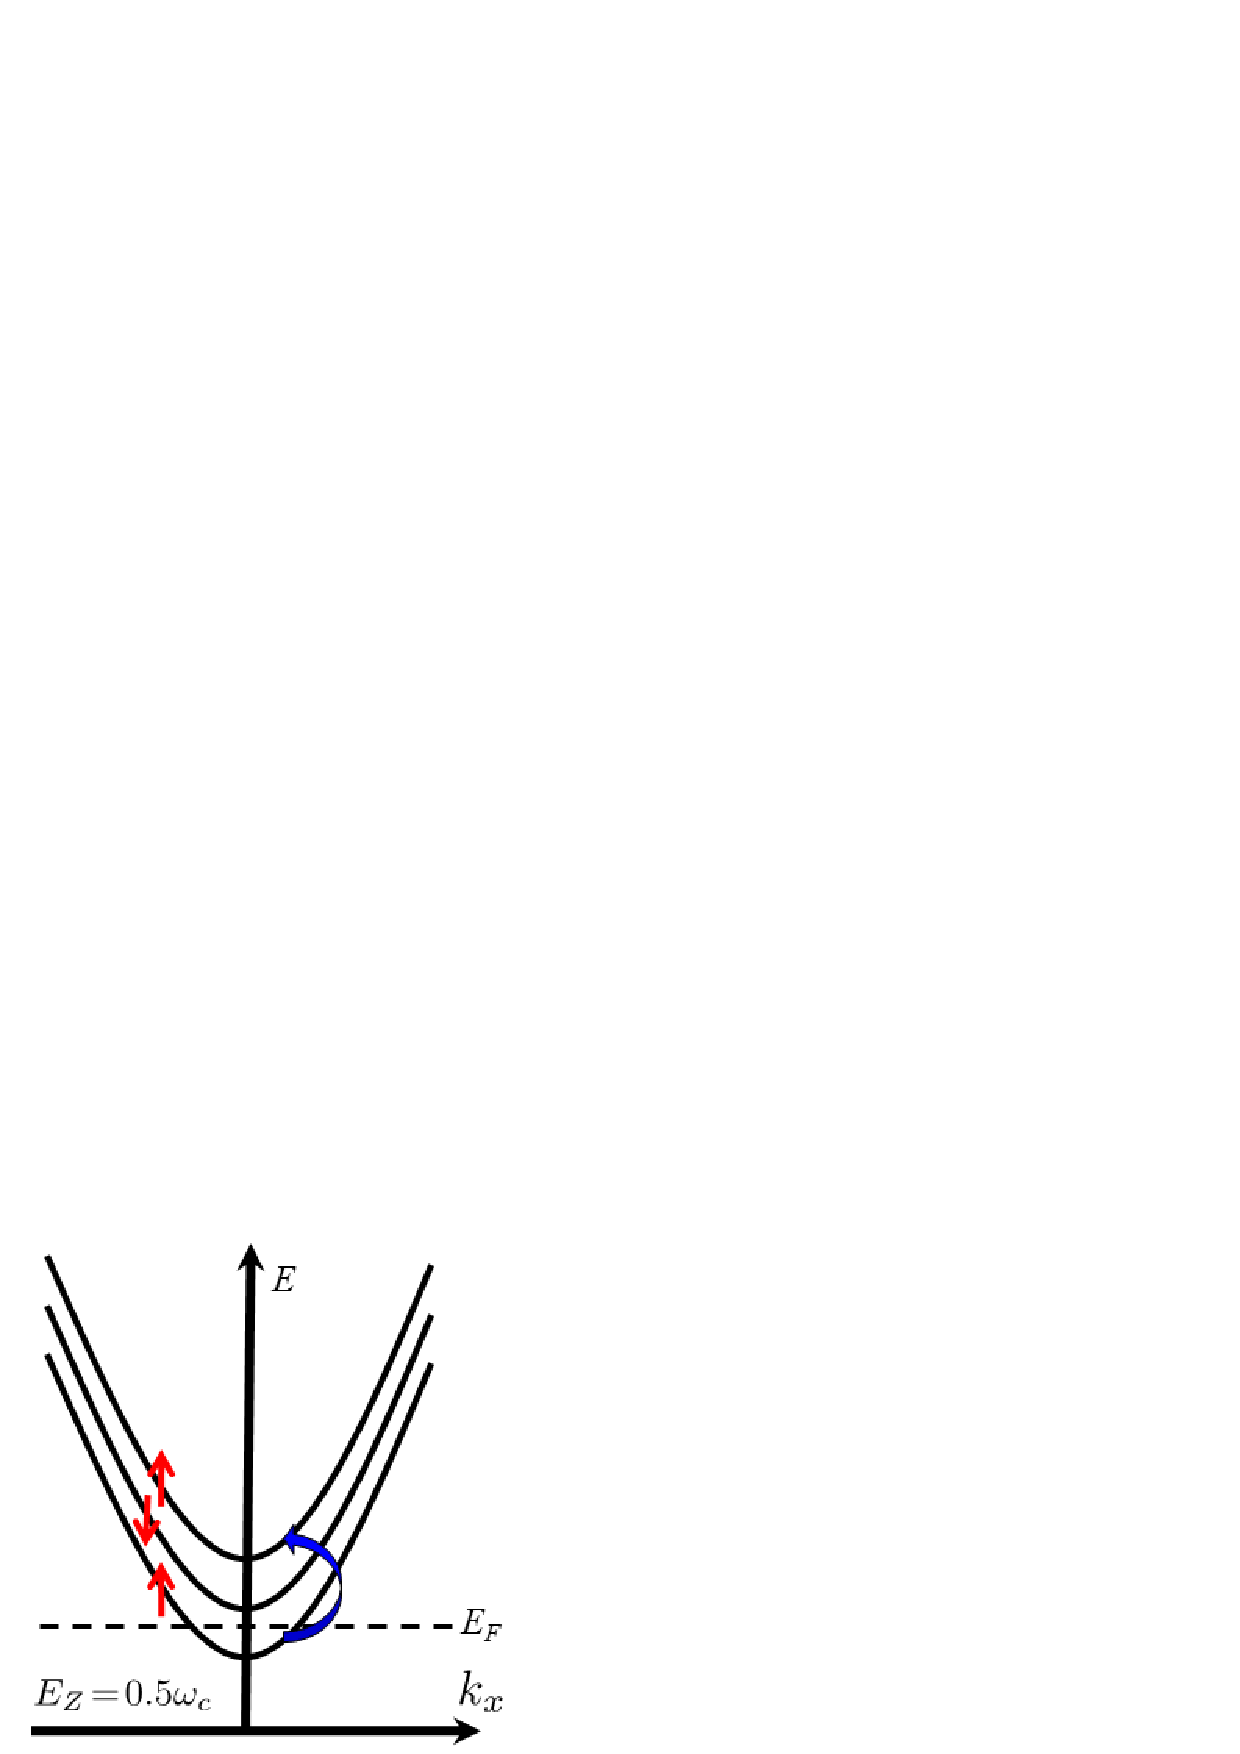
\includegraphics[width=0.7\columnwidth]{fig8.jpeg}
\caption{(color online) The three lowest energy subbands are $|0,+1\rangle$, $|0,-1\rangle$ and $|1,+1\rangle$.
The spin polarization is denoted by straight thin (red) arrows. 
Only the $|0,+1\rangle$ crosses the Fermi level, $E_F$.
The sloshing mode is the superposition of  p-h excitations from $|0,+1\rangle$ to $|1,+1\rangle$ subbands as indicated by a round thick (blue) arrow.\cite{Iqbal}}
\label{fig:par1}
\end{center}
\end{figure}



\begin{figure}[h]
\begin{center}
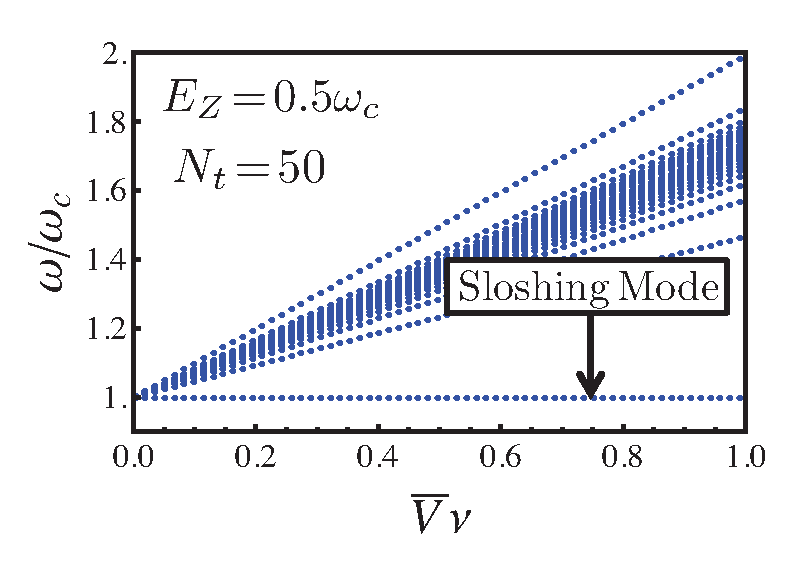
\includegraphics[width=0.6\columnwidth]{fig9.eps}
\caption{(color online) The dotted (blue) lines show the spectrum of collective modes that are the superpositions of p-h excitations between the subbands $|n+1,\pm1\rangle$ and $|n,\pm1\rangle$ as a function of the interaction parameter $\bar{V} \nu =(V_{\rho} - 3 V_s) \nu$.
The parameters used are (arb. units) $E_F = 50$,  $m=1$, $E_Z = 0.5 \omega_{\perp}$ and $\omega_{\perp} = 1$ corresponding to $N_t = 50$. 
The horizontal dotted line at $\omega/\omega_{\perp} =1$ demonstrates the Kohn theorem for sloshing mode.\cite{Iqbal}}
\label{fig:app_slosh}
\end{center}
\end{figure}




Here we demonstrate the consistency of the perturbation theory with the variants of Kohn theorem for the sloshing mode and spin precession mode.
We stress that although the perturbation theory holds for weak interaction the cancellation between the self-energy and vertex corrections holds exactly in every order of perturbation theory.
Such cancellation provides us with a test of the numerical calculations.

\section{Sloshing Mode}
Here we demonstrate the Kohn theorem for the sloshing mode in the presence of Zeeman splitting and electron-electron interaction, Eq.~\eqref{M19}.
The relevant p-h excitations are formed by the spin conserving transition between the adjacent subbands.
The electron and hole comprising such a pair reside at subbands $|n,\pm1\rangle$ and $|n+1,\pm 1\rangle$ respectively.

The most trivial is the situation with only the very lowest subband $|0,+1\rangle$ occupied, see Fig.~\ref{fig:par1}.
As only spin up species are present the short range interaction is ineffective for fermions, and the Kohn theorem is trivially satisfied.
Technically the contributions from the direct and exchange processes to both the self energy and the vertex corrections cancel.
The situation is less trivial for the large number of occupied levels.
In all cases the sloshing mode can be identified as the one not renormalized by interactions, see Fig.~\ref{fig:app_slosh}.

\begin{figure}[h]
\begin{center}
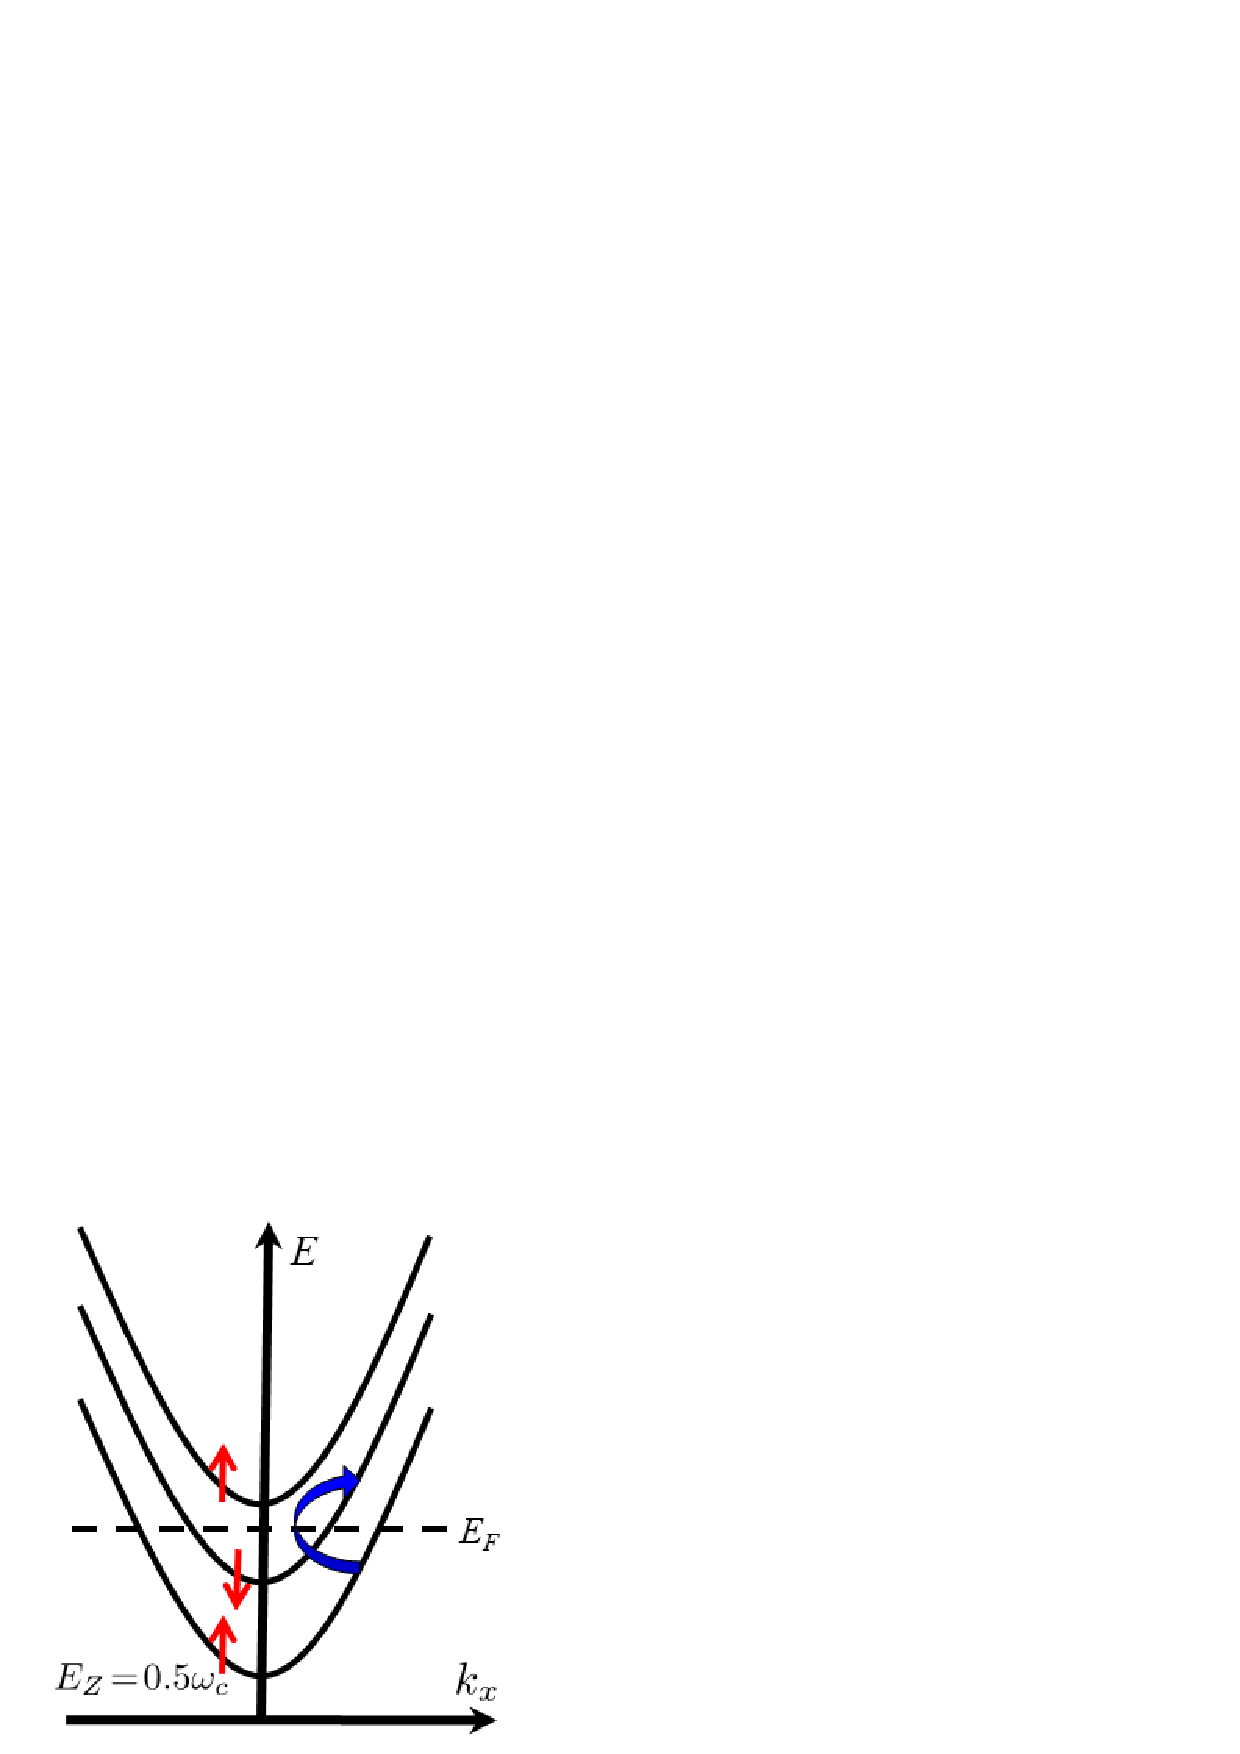
\includegraphics[width=0.4\columnwidth]{fig10.jpg}
\caption{(color online) The same three lowest energy subbands, $|0,+1\rangle$, $|0,-1\rangle$ and $|1,+1\rangle$ as in Fig.~\ref{fig:par1}.
The spin polarization is denoted by straight thin (red) arrows. 
The subbands $|0,+1\rangle$ and $|0,-1\rangle$ cross the Fermi level, $E_F$.
The spin precession mode is the superposition of  p-h excitations from $|0,+1\rangle$ to $|0,-1\rangle$ subbands as indicated by a round thick (blue) arrow.\cite{Iqbal}}
\label{fig:par2}
\end{center}
\end{figure}

\begin{figure}[t!]
\begin{center}
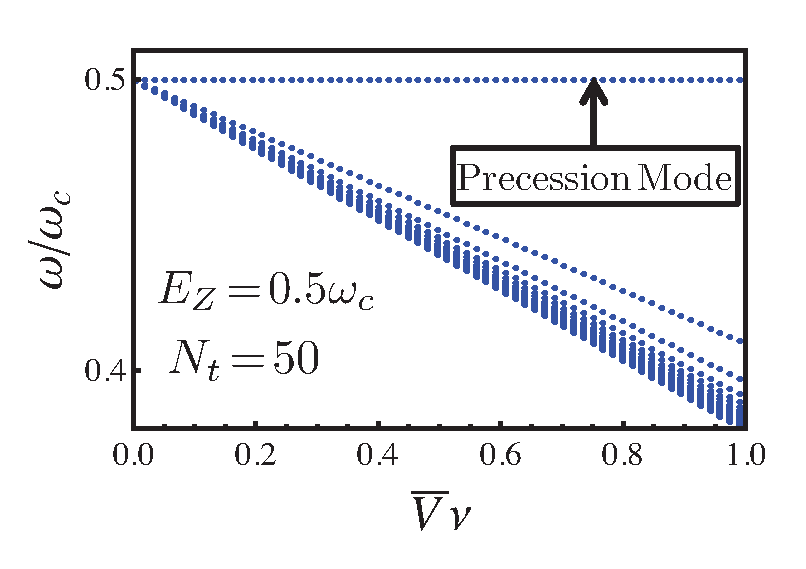
\includegraphics[width=0.6\columnwidth]{fig11.eps}
\caption{ (color online) The dotted (blue) lines show the spectrum of collective modes that are the superpositions of p-h excitations between the subbands $|n,+1\rangle$ and $|n,-1\rangle$ as a function of the interaction parameter $\bar{V} \nu =(V_{\rho} - 3 V_s) \nu$.
The parameters used are (arb. units) $E_F = 50$,  $m=1$, $E_Z = 0.5 \omega_{\perp}$ and $\omega_{\perp} = 1$ corresponding to $N_t = 50$. 
The horizontal dotted line at $\omega/ \omega_{\perp}=(\omega_{\perp} - E_Z)/\omega_{\perp} = 0.5 \omega_{\perp}$ demonstrates the Kohn theorem for spin precession mode.\cite{Iqbal}}
\label{fig:app_precession}
\end{center}
\end{figure}

\section{Spin-Precession Mode}
\label{sec:app_precession}
%
Here we make another generalization of the procedure developed in the Sec.~\ref{sec:Microscopic} to describe the effect of interactions on intra-band spin-flip transitions.
We start with the illustration of the Kohn theorem for the simplest case of two subbands occupied with Fermi momenta $k^F_{0,-1}$ and $k^F_{0,+1}$, see Fig.~\ref{fig:par2}. 
It is sufficient to focus on a single type of p-h excitations from subband $|0,+1 \rangle$ to subband $|0,-1 \rangle$.



In this case the proper generalization of the $\hat{\Gamma}$ matrix introduced in Eq.~\eqref{Gamma} has a single element,
\begin{align}\label{Gamma_app}
\Gamma(\omega) =\left[ \Pi^{-1}(\omega) + W \right]^{-1}\, ,
\end{align}
where we have for the polarization operator describing the excitations of p-h pairs shown in Fig.~\ref{fig:par2}, 
\begin{align}\label{Polarization1_app}
\Pi(\omega)= 
\frac{\pi^{-1} \left( k^F_{0,+1} - k^F_{0,-1}\right) }{
\omega  - E_Z
-
\Sigma_{0,-1} + \Sigma_{0,+1}
}
\end{align}
instead of Eq.~\eqref{Polarization1}.
The Fermi momenta and the self energies entering Eq.~\eqref{Polarization1_app} are defined by Eqs.~\eqref{kF} and \eqref{self1} respectively.
Instead of Eq.~\eqref{W} we have for the scattering vertex,
\begin{align}\label{W_app}
W =\bar{V} \ell^{-1} M^{0,0}_{0,0} \, .
\end{align}
It follow from Eq.~\eqref{Polarization1_app} that
\begin{align}\label{Polarization2_app}
\Pi^{-1}(\omega=E_Z)= 
\frac{\pi (\Sigma_{0,+1}-\Sigma_{0,-1})}{  k^F_{0,+1} - k^F_{0,-1}}\, .
\end{align}
Equation \eqref{self1} gives
\begin{align}\label{self1_app}
\Sigma_{0,\pm 1} & =
\bar{V} \ell^{-1}  \frac{k^F_{0,\mp 1}}{ \pi } M^{0,0}_{0,0}\, .
\end{align}
Combining Eqs.~\eqref{Gamma_app}, \eqref{W_app}, \eqref{Polarization2_app}, and \eqref{self1_app} we obtain
\begin{align}
\Gamma^{-1}(\omega = E_Z) = 0
\end{align}
which signifies the presence of the collective mode with unrenormalized frequency, $E_Z$ as expected.





The outlined derivation is easily generalized to arbitrary number of occupied subbands.
The condition analogous to Eq.~\eqref{det} leads to the spectrum of excitation shown in Fig.~\ref{fig:app_precession}.
The spin precession mode is identifiable as the one not renormalized by interactions.
Essentially similar approach has been used for the calculation of the spin wave dispersion in quantizing magnetic field with unequal occupation of Zeeman split Landau levels, (see Ref.~\cite{Kallin1984}).

%MK
